% Chapter 3 from the thesis template file
%   that contains an example table and figure.
\chapter{Implementation of a Software Defined Radio Radiometer}
One of the principal goals with this research was to implement a fully functioning total power radiometer within software.  The N200 provides us the link between the RF signal captured by the antenna and converts that to a format that the computer can now use to manipulate the signal.  Once the signal has been passed to the computer, GNURadio will implement the correct algorithms to detect the power within the signal, filter and output the information.  One of the advantages of course with a SDR is that filtering can also be done within the software.  In addition, thanks to the WxGUI that GNURadio uses, we can also build a user interface that can control several key variables that are useful for us.  This includes controlling the gain on the programmable gain amplifier on the DBSRX2 card, the sampling or bandwidth of the signal, the center frequency, and also the integration time.  All of these can now be controlled in real time as well.  GNURadio will also store the power data so that we are able to do further analysis of the data using a software program like MatLab.  Because GNURadio is a very flexible system, much more can be done with the signal if needed and future updates may add more capabilities or additional analysis on the signal can be achieved.

\section{Requirements}

Requirements for this system was based largely on what the current ISU radiometer was capable of doing and was also based on requirements of a typical radiometer.  These requirements are outlined in table~\ref{requirements} below.


\begin{table}[h!tb] \centering
\isucaption{ISU Radiometer requirements}
\label{requirements}
\begin{tabular}{lcc} \hline
\textbf{Requirement} & \textbf{Value} & \textbf{Units} \\ \hline
Frequency Range & 1400 - 1425 & MHz \\
Bandwidth & 25 & MHz \\
Polarization & Dual &  \\ 
Sensitivity & -30 & dBm \\
Accuracy & 1 & Kelvin \\ \hline
\end{tabular}
%\vspace{ 2 in}
\end{table}

\subsection{Hardware Requirements}

The selection of the N200 SDR from Ettus Research was based on many of the requirements outlined in table~\ref{requirements}.  In addition, we wanted the hardware to be flexible but also affordable.  There are many different kinds of software defined radios on the market.  However, we choose the N200 based on the availability of the device, the large community support, especially with regards to support by GNURadio, and because it meet and often exceeded the requirements stated above.  

Flexibility was another key aspect of the N200 that made it an excellent selection for this research.  The N200 uses a daughter board setup for bridging the RF interface to the rest of the electronics.  Several different daughter boards are available that have different frequency ranges and offer both receive, transmit and transceiver designs.  For the radiometer we need to operate around 1.4 GHz and receive only.  Based on those requirements we choose the DBSRX2 daughter board.  This board is designed from 800 MHz to 2.3 GHz and has a fairly low noise figure.   

The current RF front end to the radiometer is designed for a 20 MHz wide signal.  This requirement was one of the main driving points for selecting the N200 SDR as it can support up to 50 MHz in bandwidth between the N200 and the host computer.  This is accomplished by using a 1 Gbps Ethernet connection between the N200 and the host computer.

\subsection{Software Requirements}

The driving force for the software requirement was to have a system that was easy to use.  The ISU radiometer originally used LabWindows, to retrieve data and control the radiometer.  A revision was made that changed the interface control to LabView.  In both cases the interface was a graphical interface that allowed the user to easily set parameters and download the data.

The original ISU Radiometer did most of it's processing on board the FPGA which ran custom firmware provided by the University of Michigan.  The graphical interface simply downloaded the data and allowed for control of certain parameters.  However, since the RF front end used traditional components, there was very little that could be changed in the RF chain.  With the switch to a software defined radio platform, we switched to having most of the processing done by the host computer with digitization and low level processing accomplished by the software defined radio's FPGA.  However, we still wanted to keep the interface hardware fairly simple.  GNURadio was selected as it includes GNURadio Companion (GRC) which uses a graphical interface for creating the radio environment.  It also includes options to create a user interface during the operation of the N200 as well.  This allowed us to rapidly create both the critical radio components needed for the radiometer and also a control interface.

\section{Power detection}
Power detection is a key ability that allows a radiometer to function.  At its core a radiometer is a power detector.  Therefore the implementation of power detection is a crucial function of a software defined radio radiometer.

To implement a total power radiometer in software, we first need to look at how we implement a total power radiometer traditionally.  Traditionally, a square law detector is used to detect the average power that is seen by the radiometer.  This simple device uses a diode that gives a small voltage output based on the RF power present.  This small voltage is then amplified and can now be calibrated with a known source to give us a noise temperature.  

{\begin{figure}[h!tb] 
\centering
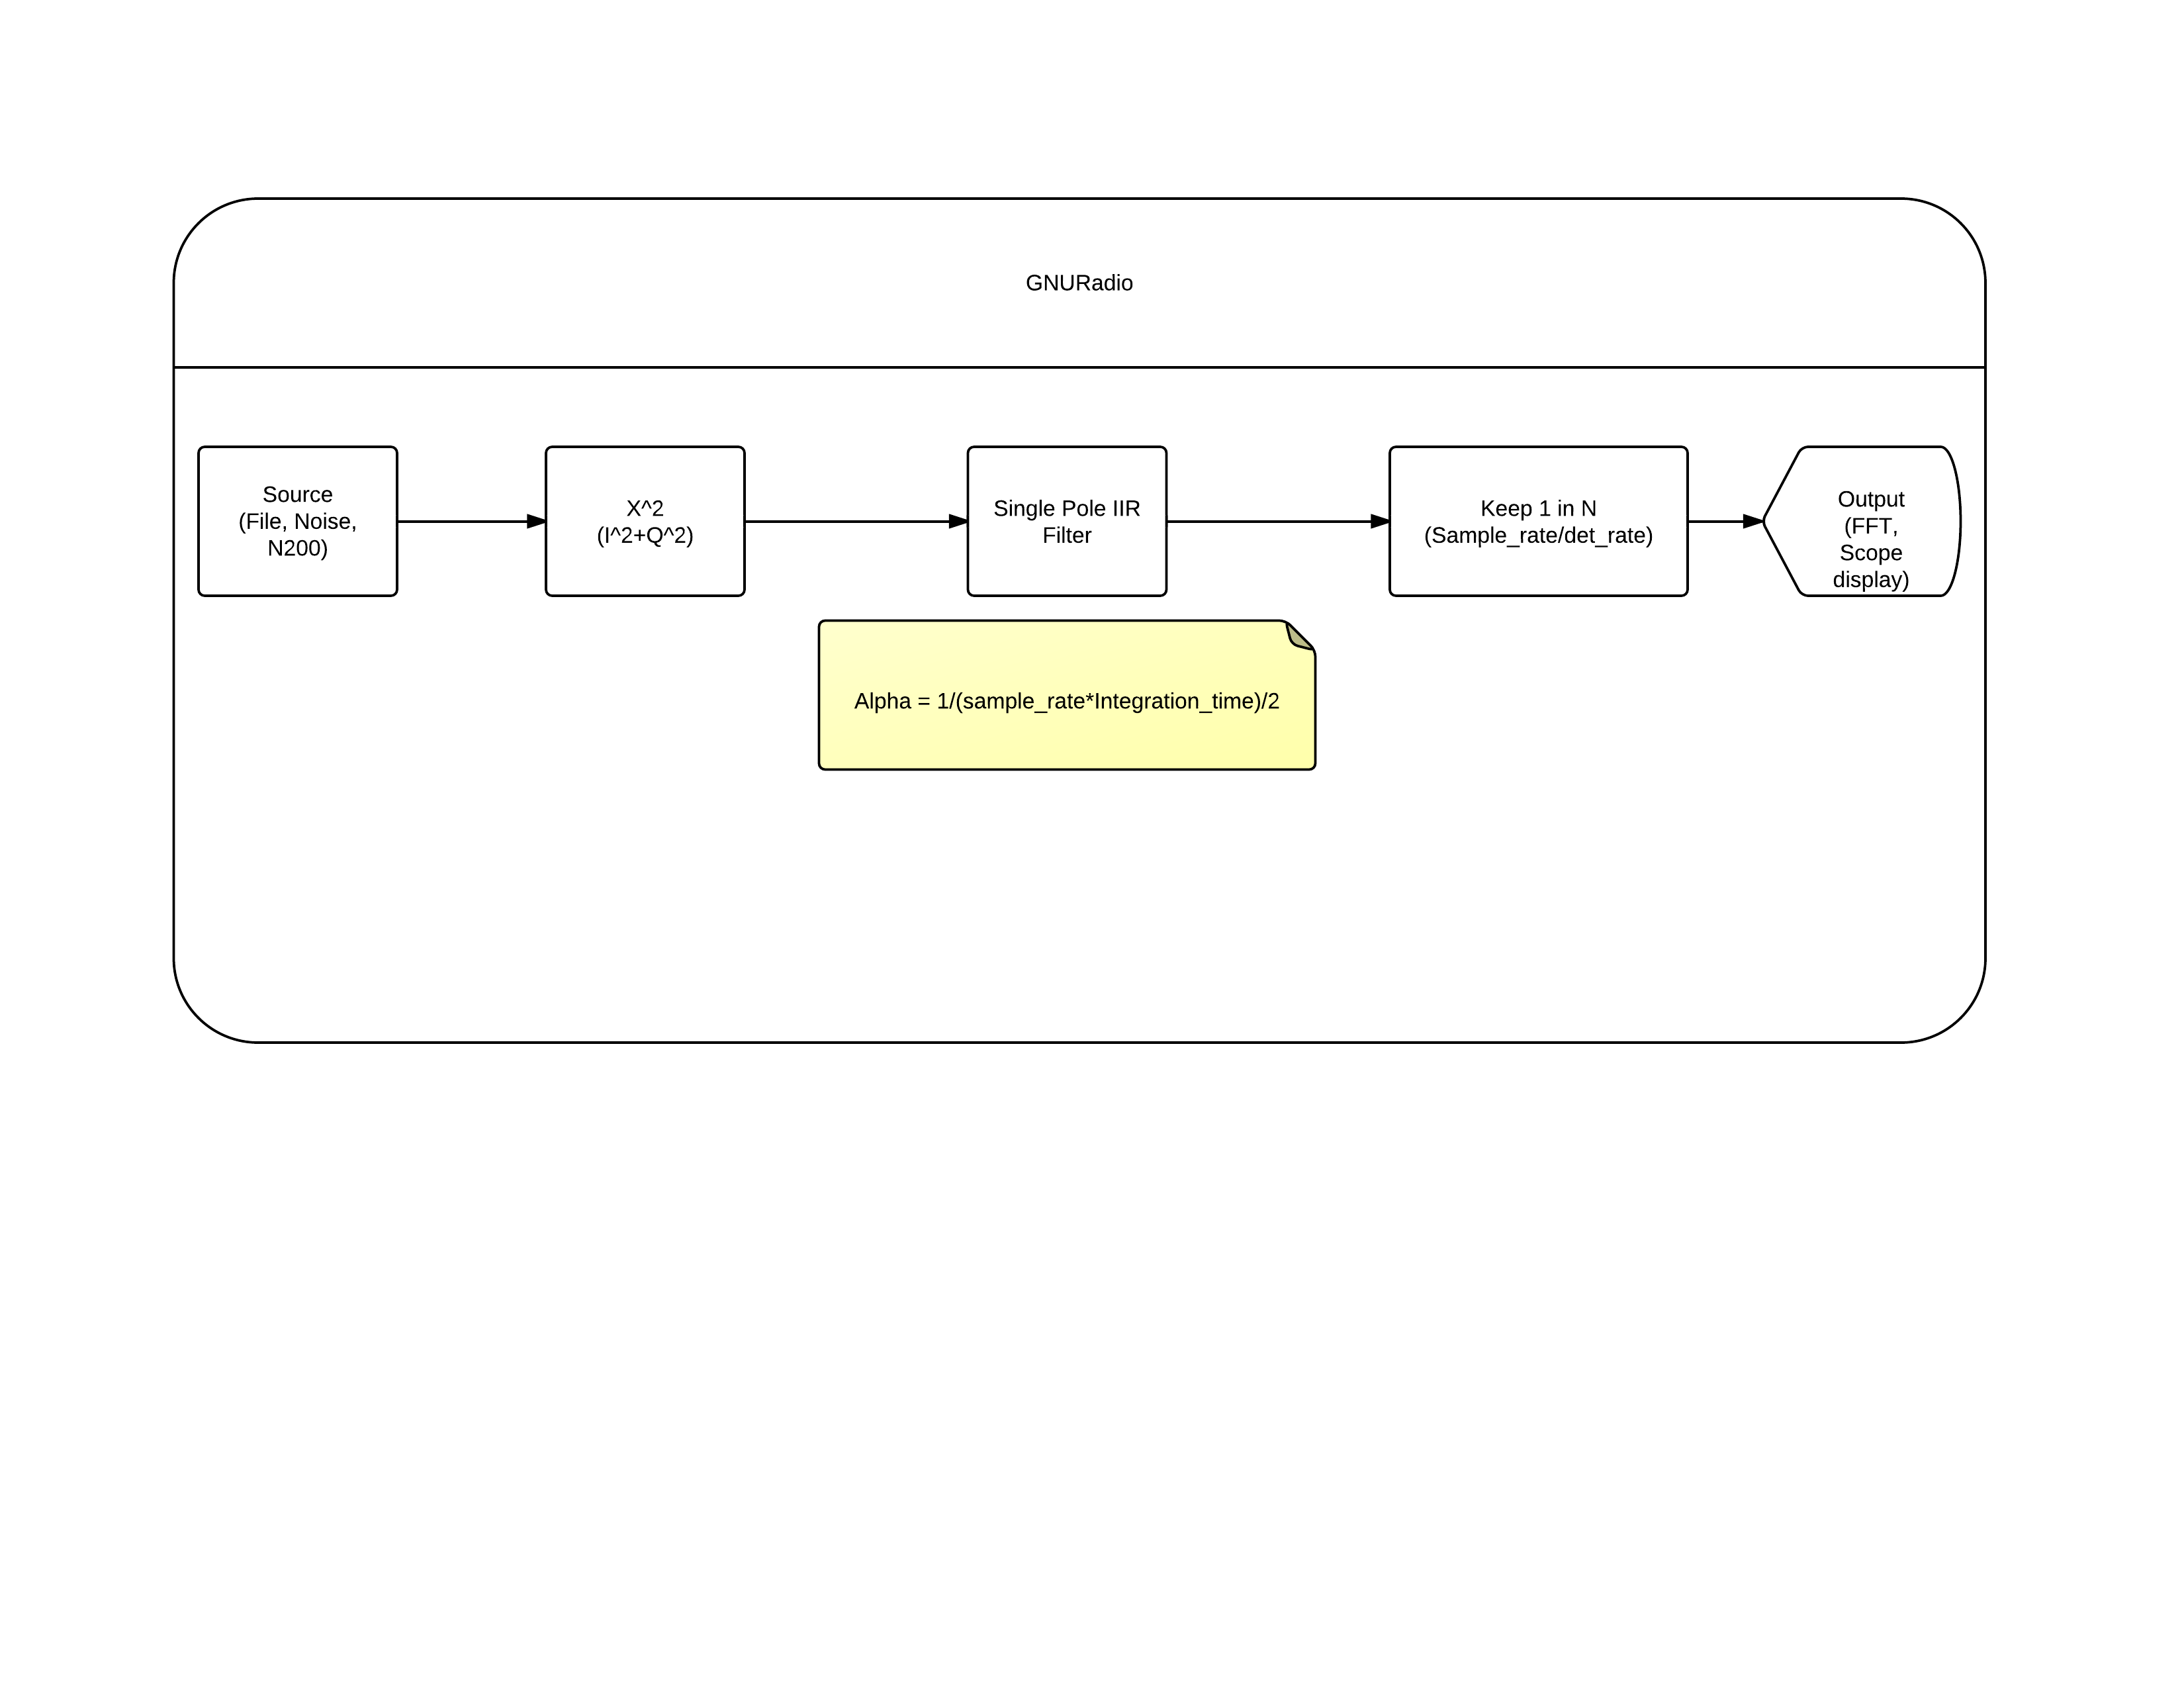
\includegraphics[width=17cm]{Images/GNURadio_Block.png}
\isucaption{A block diagram showing how the radiometer performs the equivalent square law detector in software.}
\label{square_block}
\end{figure}
}

To implement this in software, we need to build a square law detector mathematically.  We can then give this to the software defined radio to process the information accordingly.  A square law detector mathematically, is the sum of the squares.  Once the signal has been digitized, it is expressed in data bits of I and Q, which represent in-phase and quadrature-phase of the signal.  By squaring each term, we get the desired result of the power of the signal [\cite{Sarijari}][\cite{Rashid}].

\section{Integrator through a IIR Filter}

Another step that we typically do in a traditional radiometer is to integrate the signal over time.  This gives us an average of the signal and helps to smooth out the output.  In addition, we will show later that the integration time can be adjusted to help improve our sensitivity of the radiometer.

In a traditional radiometer can integrate by using a simple integrator circuit, which consists of an op-amp, resistor and capacitor.  This type of circuit is also equivalent to a low pass filter circuit as well, and the two are interchangeable.  We can then look at how we filter in the digital domain, and this is down with a infinite impulse response filter or IIR.  We can use this type of digital filter to then integrate the signal for our total power radiometer. 

\section{GNURadio Blocks}
A software defined radio by its definition requires software for the proper operation of the radio.  In our case there is the software or firmware that resides on the FPGA and then the software that runs on the computer.  For this thesis, we focused on the software running on GNURadio.  This software package provides us with the ability to write the code needed to implement a total power radiometer but also gives us a method to control the SDR as well.  It also allows for us to record the information for performing post-processing on the data.

\section{Control of the SDR Hardware through GNURadio}
The N200 sends all data across the 1 Gbps connection to be read in by a host computer running GNURadio.  This data is the raw I/Q values that is read by the on board A/D and processed by the on board FPGA.  An example of a very simple GNURadio software implementation would simply take this data and store the data to a hard drive in a file.  This can be very handy if we want to simply record the data and then process it later.  However, depending on the sample rate, it can consume a large amount of storage.  A short recording can easily consume 1-2 GB with a sample rate of 10 Msps.  It also does not give us any immediate feedback on the radiometer and it does not give us controls of the radiometer such as frequency, integration time or other key variables.  Fortunately GNURadio has tools that allows us to build up a very rich application that is able to give us the data we need and control the software defined radio as well.

The GNURadio Companion allows us to create python code that is used to not only receive the data from the SDR but also perform calculations, signal processing and also to send control information to the SDR.  This allows us to build up an application that can be run on any computer that is capable of running GNURadio.  

{\begin{figure}[h!tb] 
\centering
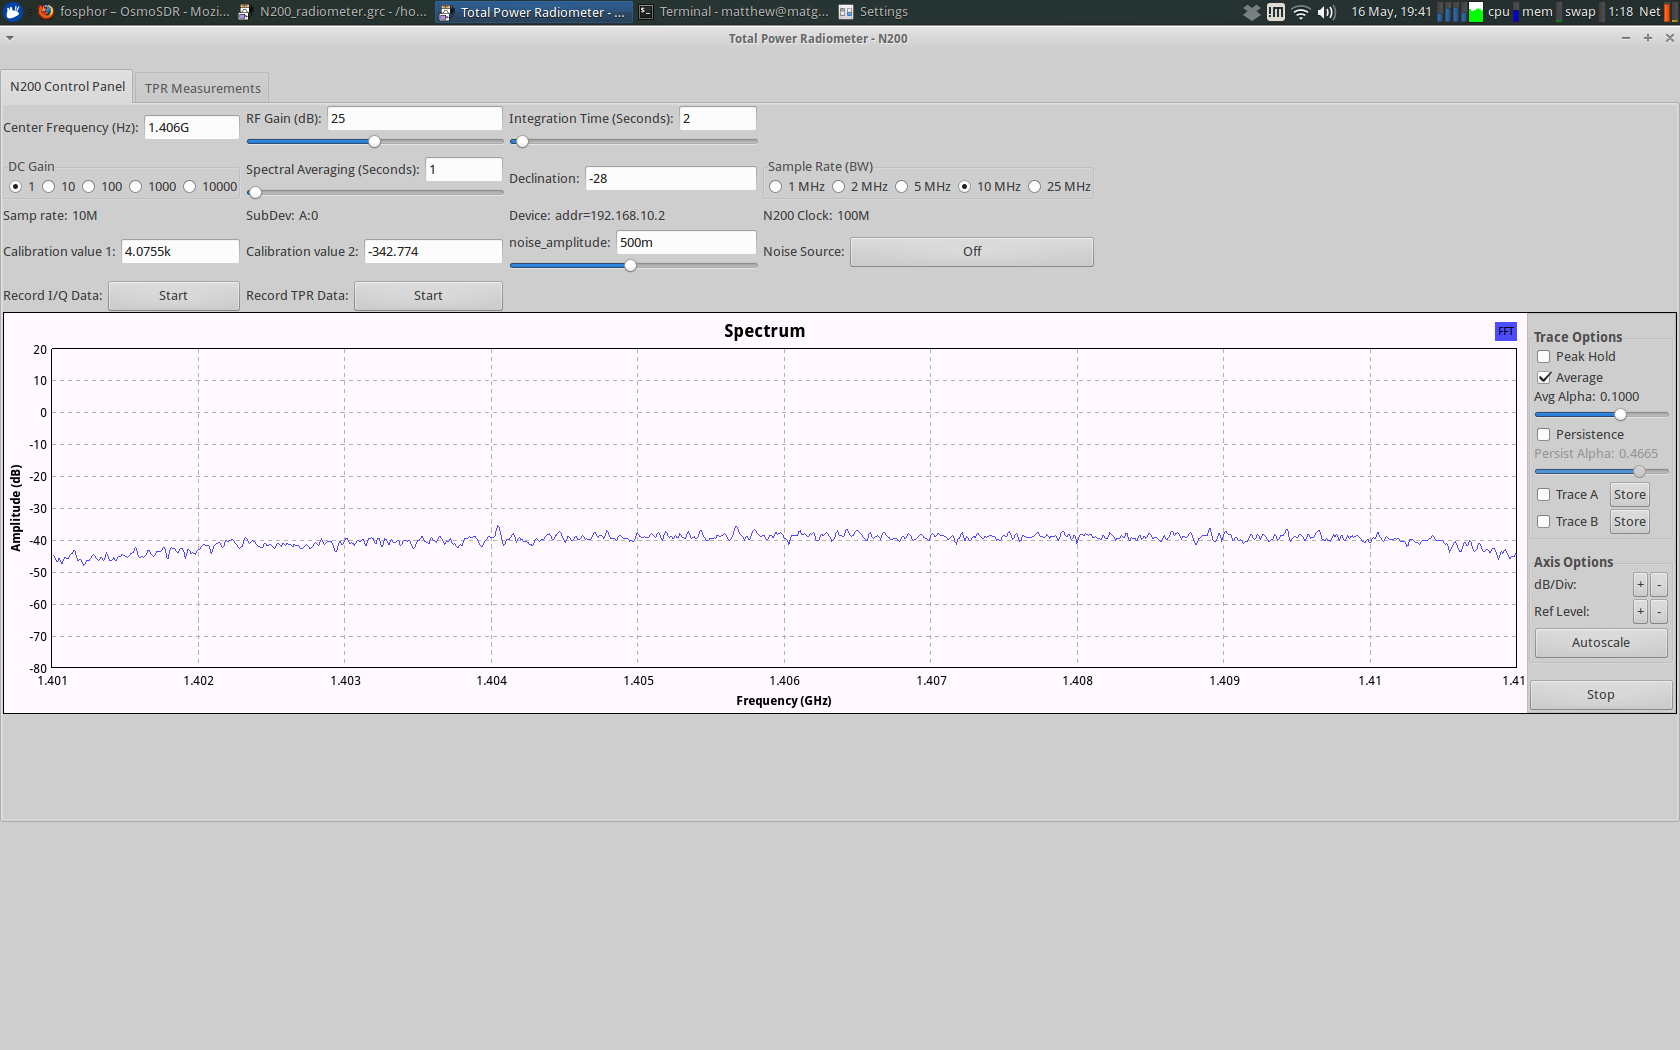
\includegraphics[width=17cm]{Images/radiometer_gui.png}
\isucaption{A screenshot of the interface made for communication with and controlling the software defined radio}
\label{radiometer_gui}
\end{figure}
}

Through this interface we are able to control several key aspects of not only the radio hardware within the SDR but also with the behavior of the radiometer as well.  Hardware control of the SDR hardware allows us to change frequency and also adjust gain values within the N200.  Bandwidth is another parameter that can be altered from here as well.  Bandwidth affects the bandwidth for the RF signal, but also has an impact on the radiometer sensitivity as well.  Additional controls allows for alterations to the radiometer and includes being able to adjust the integration time of the radiometer.  

\section{GNURadio Data Handling}
Once we have the data that has been processed by the software defined radio, we will want to display this information and be able to store the data so we can analyze it later if needed.  Data display can be handled GNURadio, where we can plot the total power over time.  This allows the user to be able to visualize the total power and be able to determine if the total power has increased or decreased over the time window shown.  

Although not usually needed for a total power radiometer, we also have the ability to look at the signal in terms of a frequency versus amplitude.  This allows to look for any unusual signals that may be interfering with or causing erroneous data with our radiometer.  

Finally we will want to store the data so we can do additional analyses on it at a later time.  The GNURadio program allows us to store the data in two formats.  The first format is storing the raw I/Q data from the radiometer.  This format allows us to "playback" the data through GNURadio at a later time.  This can be useful for if we wish to change parameters in GNURadio such as bandwidth or integration time.  It can also be a good diagnostic tool as we can check that the signal coming in is clean or if we need to apply additional filters to remove an unwanted signal. It should be noted that this file can be quite large, consuming several gigabytes of data for a 20 MHz wide signal in a matter of minutes of record time.

The second format is the total power that has been calculated by the radiometer.  This file is much smaller in size since much of the signal information has now been reduced to simple power versus time information.  This allows for easy manipulation through any type of math program such as Matlab for analysis.  

\subsection{GNURadio Data Display}
The information from the software defined radio can be displayed through GNURadio to show a number of things.  Since we have both frequency and magnitude information we can display this information.  We are able to also display the information that shows the total power that is being seen by the radiometer as well.

{\begin{figure}[h!tb] 
\centering
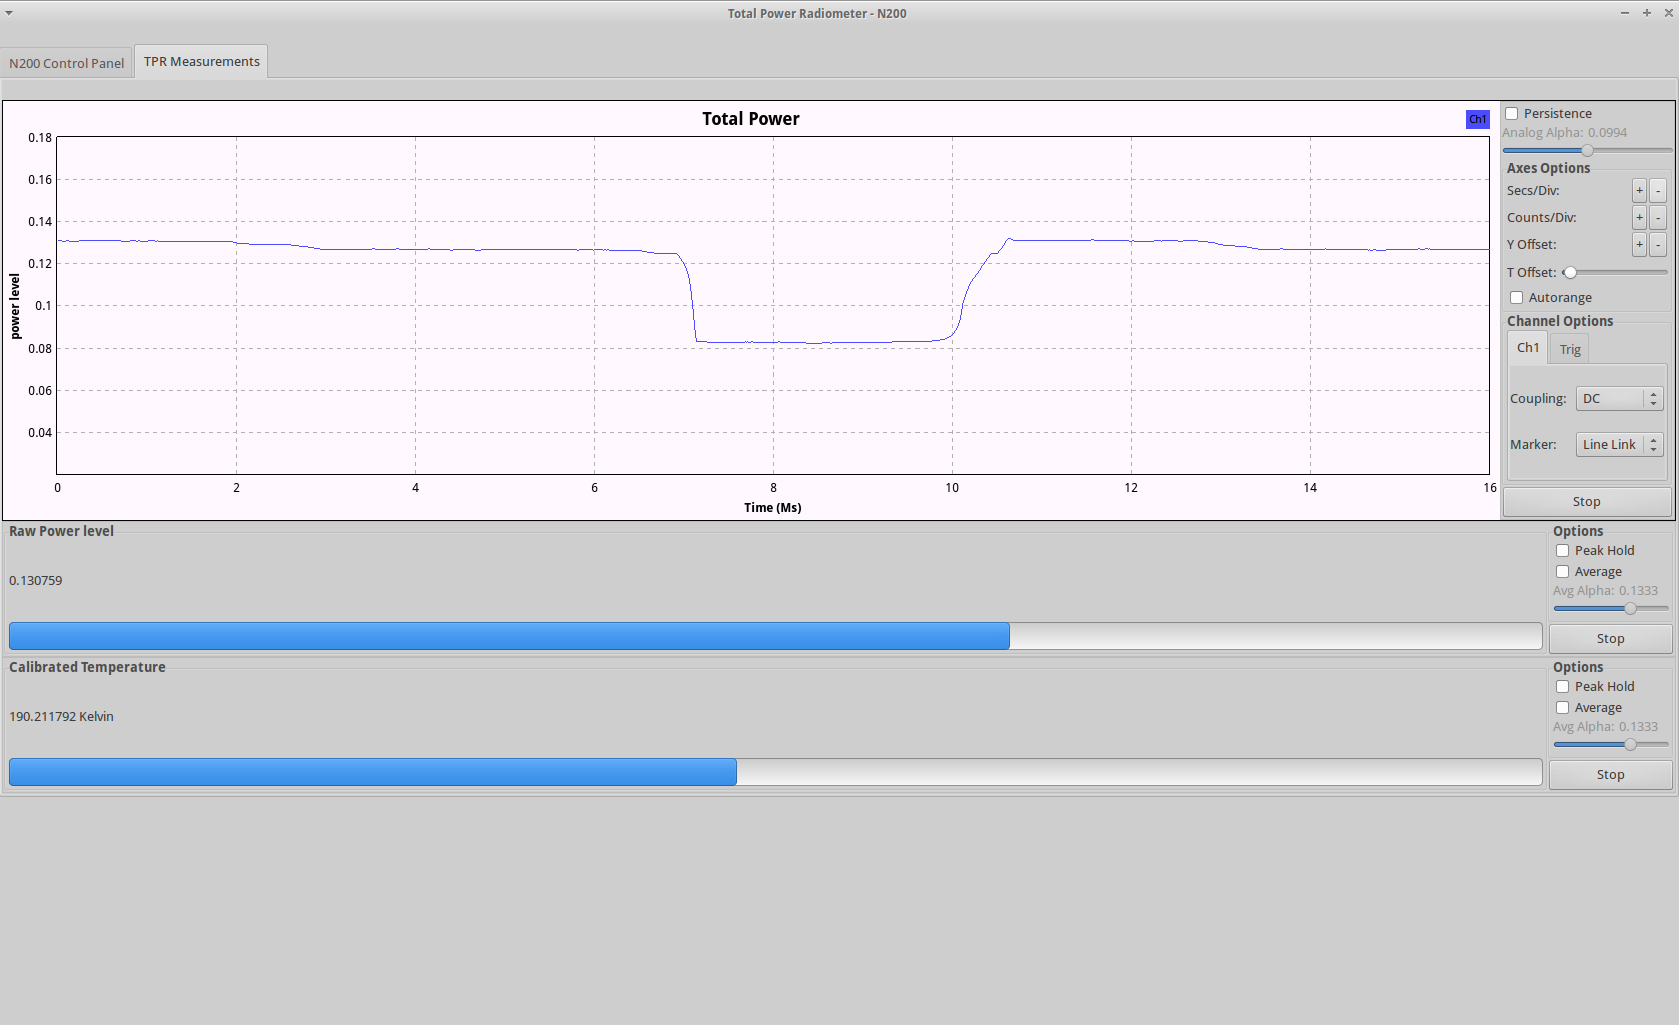
\includegraphics[width=17cm]{Images/Lab1_TPR_at_end_exp.png}
\isucaption{A screenshot showing the ticker tape display for the total power readings.  In addition raw and calibrated noise temperature is shown below.}
\label{radiometer_tpr_display}
\end{figure}
}

We are not limited to just total power from the radiometer.  If the radiometer has been calibrated, those calibration points can be entered and GNURadio can calculate the calibrated noise temperature.  Additional information may also be added as needed.  For example, we are able to view the full spectrum that the radiometer sees.  This can be a useful tool for looking at potential RFI issues.    

\subsection{GNURadio Data Processing}

GNURadio is capable of storing information in files that can be processed later.  These files are binary formats that are stored in a little-endian format and can be a character, integer, float or complex.  A simple example is storing the raw I/Q values to a file.  This file can then be processed by Python, GNURadio, or even Matlab.  For example, we can store the raw I/Q values and then play them back though GNURadio.  Of course other information can be stored as well and we use this same method to store the total power radio values to a file as well.  

{\begin{figure}[h!tb] 
\centering
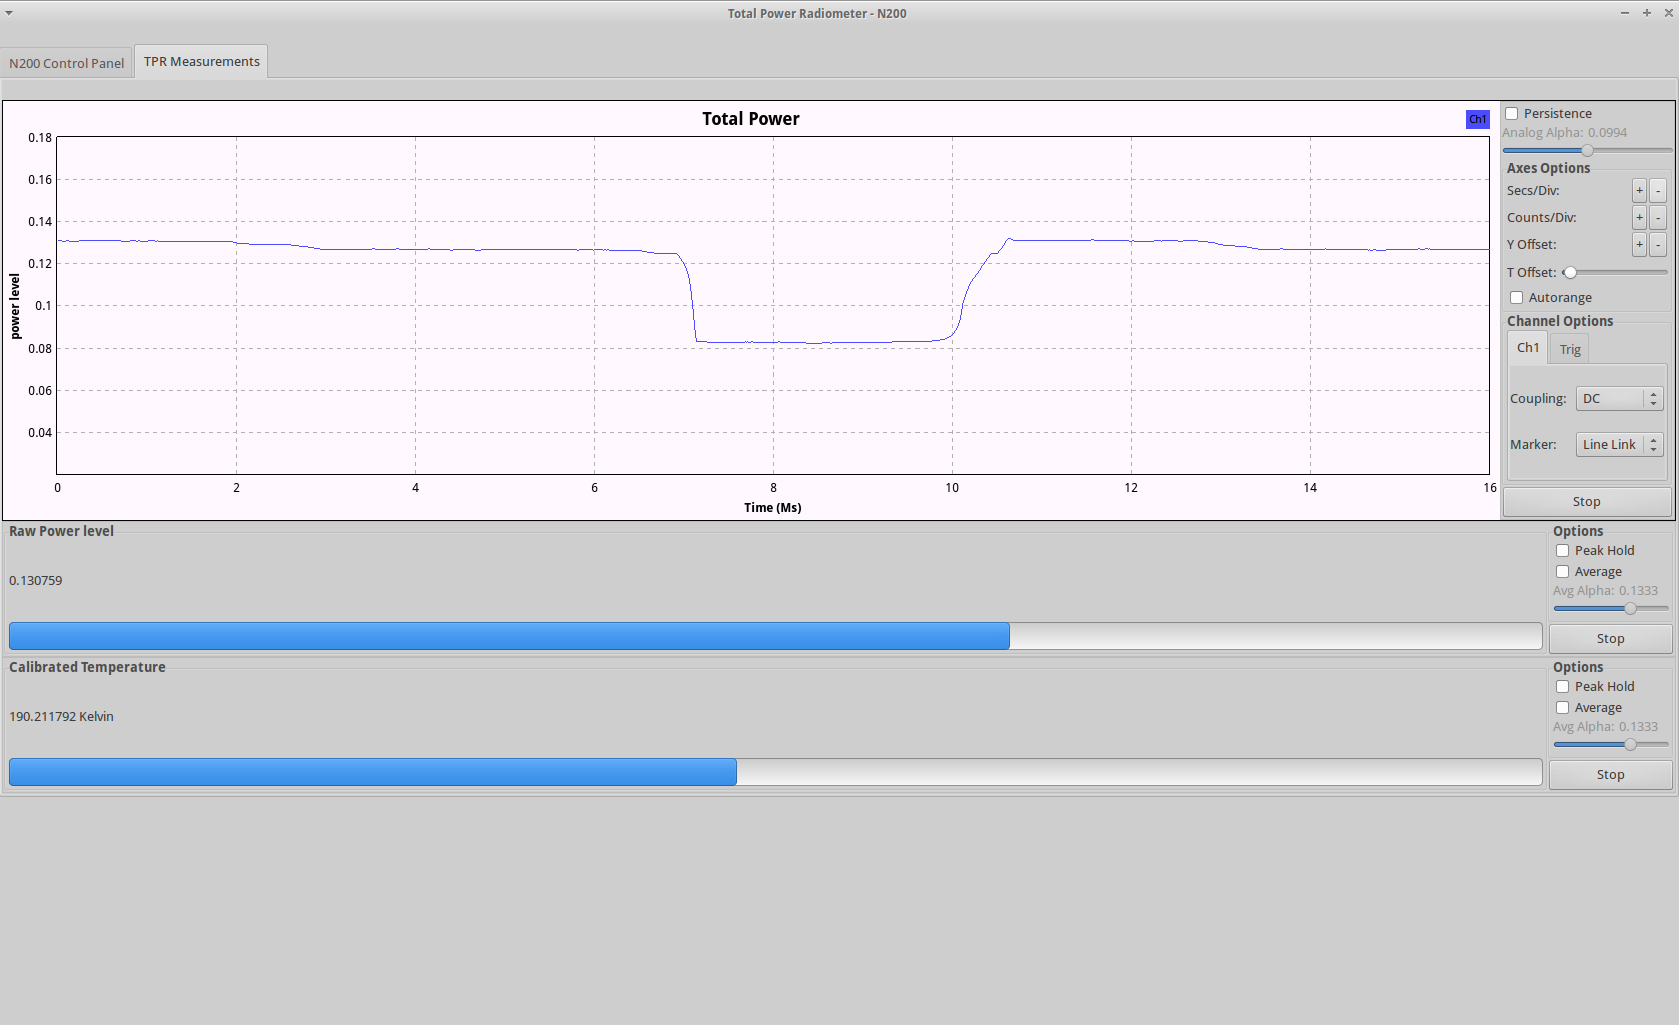
\includegraphics[width=17cm]{Images/Lab1_TPR_at_end_exp.png}
\isucaption{A screenshot showing the Matlab code and related graphs generated}
\label{radiometer_tpr_display}
\end{figure}
}

Matlab is one tool we can use to process the information that is stored by GNURadio.  Appendix A contains the Matlab source that will read the total power file generated by GNURadio.  It then calculates information such as the NE $\Delta$ T and the calibration points based on the user input.  We can also use Matalb to graph this information as well.


%Commented out for now, may place elsewhere
%\section{Hardware}
%There are two main hardware components that make up the radiometer.  The first and probably the most critical is the RF front end of the radiometer.  This critical component is what reads the RF coming in from the antenna or source.  It is then amplified so that it can then be processed.  Processing is then handled by the software defined radio, which digitizes the signal so it can be processed by the on-board FPGA and computer.  As we will discuss next, due to noise temperature considerations, we need to make sure the incoming RF signal is as noise free as possible so we are able to process the signal that we want.  



%\subsection{Noise Temperature Consideration}


%\begin{equation}
%NE\Delta T=\frac{T_{A}+T_{sys}}{\sqrt{\beta * \tau}}%For any radiometer noise temperature is a large consideration and is critical to the design of the radiometer.  One method to determine how well a radiometer is to look at the sensitivity of the radiometer.  We can do this by looking at the smallest change in temperature the radiometer can see.  We will call this the Noise Equivalent $\Delta T$ or $NE\Delta T$ of the radiometer.  The equation for this is shown below.

%\end{equation}

%For our radiometer, we will assume that our bandwidth, $\beta$, is fixed at 20 MHz.  This is due to the current RF hardware that is placed in front of the N200 which has band-pass filters that restrict the incoming signal to between 1.400 and 1.420 GHz. 

%Need to add information about the ISU Radiometer antenna and what it adds to the noise temperature

%For $T_{sys}$, both the RF front end and the software defined radio needs to be included and calculated to see the impact to the overall $NE\Delta T$ of the radiometer.  

%Finally $\tau$ is the integration time for the radiometer.  This parameter is set by the user and is the only variable that we have direct control of.  

%\subsection{DBSRX2 Noise Temperature Consideration}

%The N200 uses daughter board cards that allow for us to easily swap out different RF front ends.  The DBSRX2 was selected due to the fact that it is receive only and that it will work in the frequency spectrum that we are interested in, primarily in the 1.4 GHz range.  Since we are using the DBSRX2 after the LNAs that are already on the, the noise temperature added by the DBSRX2 will be quite small.  The DBSRX2 adds approximately 5 dB to the noise factor of the system.  Again though, since this is at the end of the RF chain, the total contribution of the DBSRX2 to the overall system noise temperature is small, and has been calculated to be 1.05 dB to the overall noise factor of the system.

%While the DBSRX2 does have additional gain, this gain is not as critical since we have the additional gain from the ISU radiometer front end.  While the gain the DBSRX2 is significant, the noise figure on the DBSRX2 by itself is quite high.  Therefore, the DBSRX2 would not be a good candidate if the N200 would be used solely by itself.  Ideally, there would be at least one if not multiple LNA's that have much better noise figure numbers than what the DBSRX2 and would be placed in front of the DBSRX2 daughter-board.  

%The filters that are on the ISU radiometer are not as critical and, in fact, could be removed.  Once we have the signal in the digital domain, it is possible to build and even adjust band-pass filers in software instead of using hardware. This can have the advantage of reducing some of the noise that these band-pass filters add, although their contribution is small.  One drawback to this however is that it will require additional computation cycles.  In our case, since the ISU radiometer already has band-pass filters, we assume the signal will be valid in that range.  We do however, artificially apply a band-pass to the system in software by defining the sample rate that we receive the data from the N200.  For this reason, we do need to know what our sample rate is, as often that will be smaller than the bandwidth coming from the ISU radiometer. 

